\documentclass[table,xcolor=table]{IFMG-beamer}

% --------------------------------------------------- %
%                  Informações      	              %
% --------------------------------------------------- %
\title[Minha apresentação]{Minha apresentação em LaTeX}
\subtitle{Subtítulo}
\author{Meu nome}
\institute[IFMG]{Instituto Federal de Minas Gerais\\
  Campus Ibirité
}
\date[\today]{}


\subject{Meu tema } % metadata

% --------------------------------------------------- %
%                    Title + Schedule                 %
% --------------------------------------------------- %

\begin{document}

\bgroup
\setbeamertemplate{navigation symbols}{}
\makeatother
\bgroup

\setbeamertemplate{footline}
{
  \leavevmode%
  \hbox{%
  \begin{beamercolorbox}[wd=.2\paperwidth,ht=2.25ex,dp=1ex,center]{author in head/foot}%
    \usebeamerfont{author in head/foot}\insertshortauthor%\expandafter\beamer\ifempty\expandafter{\beamer\shortinstitute}{}{~~(\insertshortinstitute)}
  \end{beamercolorbox}%
  \begin{beamercolorbox}[wd=.65\paperwidth,ht=2.25ex,dp=1ex,center]{title in head/foot}%
    \usebeamerfont{title in head/foot}\insertshorttitle
  \end{beamercolorbox}%
  \begin{beamercolorbox}[wd=.15\paperwidth,ht=2.25ex,dp=1ex,center]{date in head/foot}%
    \usebeamerfont{date in head/foot}\insertshortdate{}%\hspace*{2em}
%    \insertframenumber{} / \inserttotalframenumber\hspace*{2ex} 
    %\hspace*{6ex}
  \end{beamercolorbox}}%
  \vskip0pt%
}


\begin{frame}
    \maketitle
\end{frame}


\egroup

\setbeamertemplate{footline}
{
 \leavevmode%
  \hbox{%
  \begin{beamercolorbox}[wd=.2\paperwidth,ht=2.25ex,dp=1ex,center]{author in head/foot}%
    \usebeamerfont{author in head/foot} \insertshortauthor{}
  \end{beamercolorbox}%
  \begin{beamercolorbox}[wd=.65\paperwidth,ht=2.25ex,dp=1ex,center]{title in head/foot}%
    \usebeamerfont{title in head/foot}\insertshorttitle
  \end{beamercolorbox}%
  \begin{beamercolorbox}[wd=.15\paperwidth,ht=2.25ex,dp=1ex,right]{date in head/foot}%
    %\usebeamerfont{date in head/foot}\insertshortdate{}\hspace*{2em}
    \insertframenumber{} %/ \inserttotalframenumber
    \hspace*{6ex}
  \end{beamercolorbox}}%
  \vskip0pt%
}


%LOGO
\addtobeamertemplate{frametitle}{}{%
\begin{textblock*}{10mm}(11.5cm,-0.75cm)
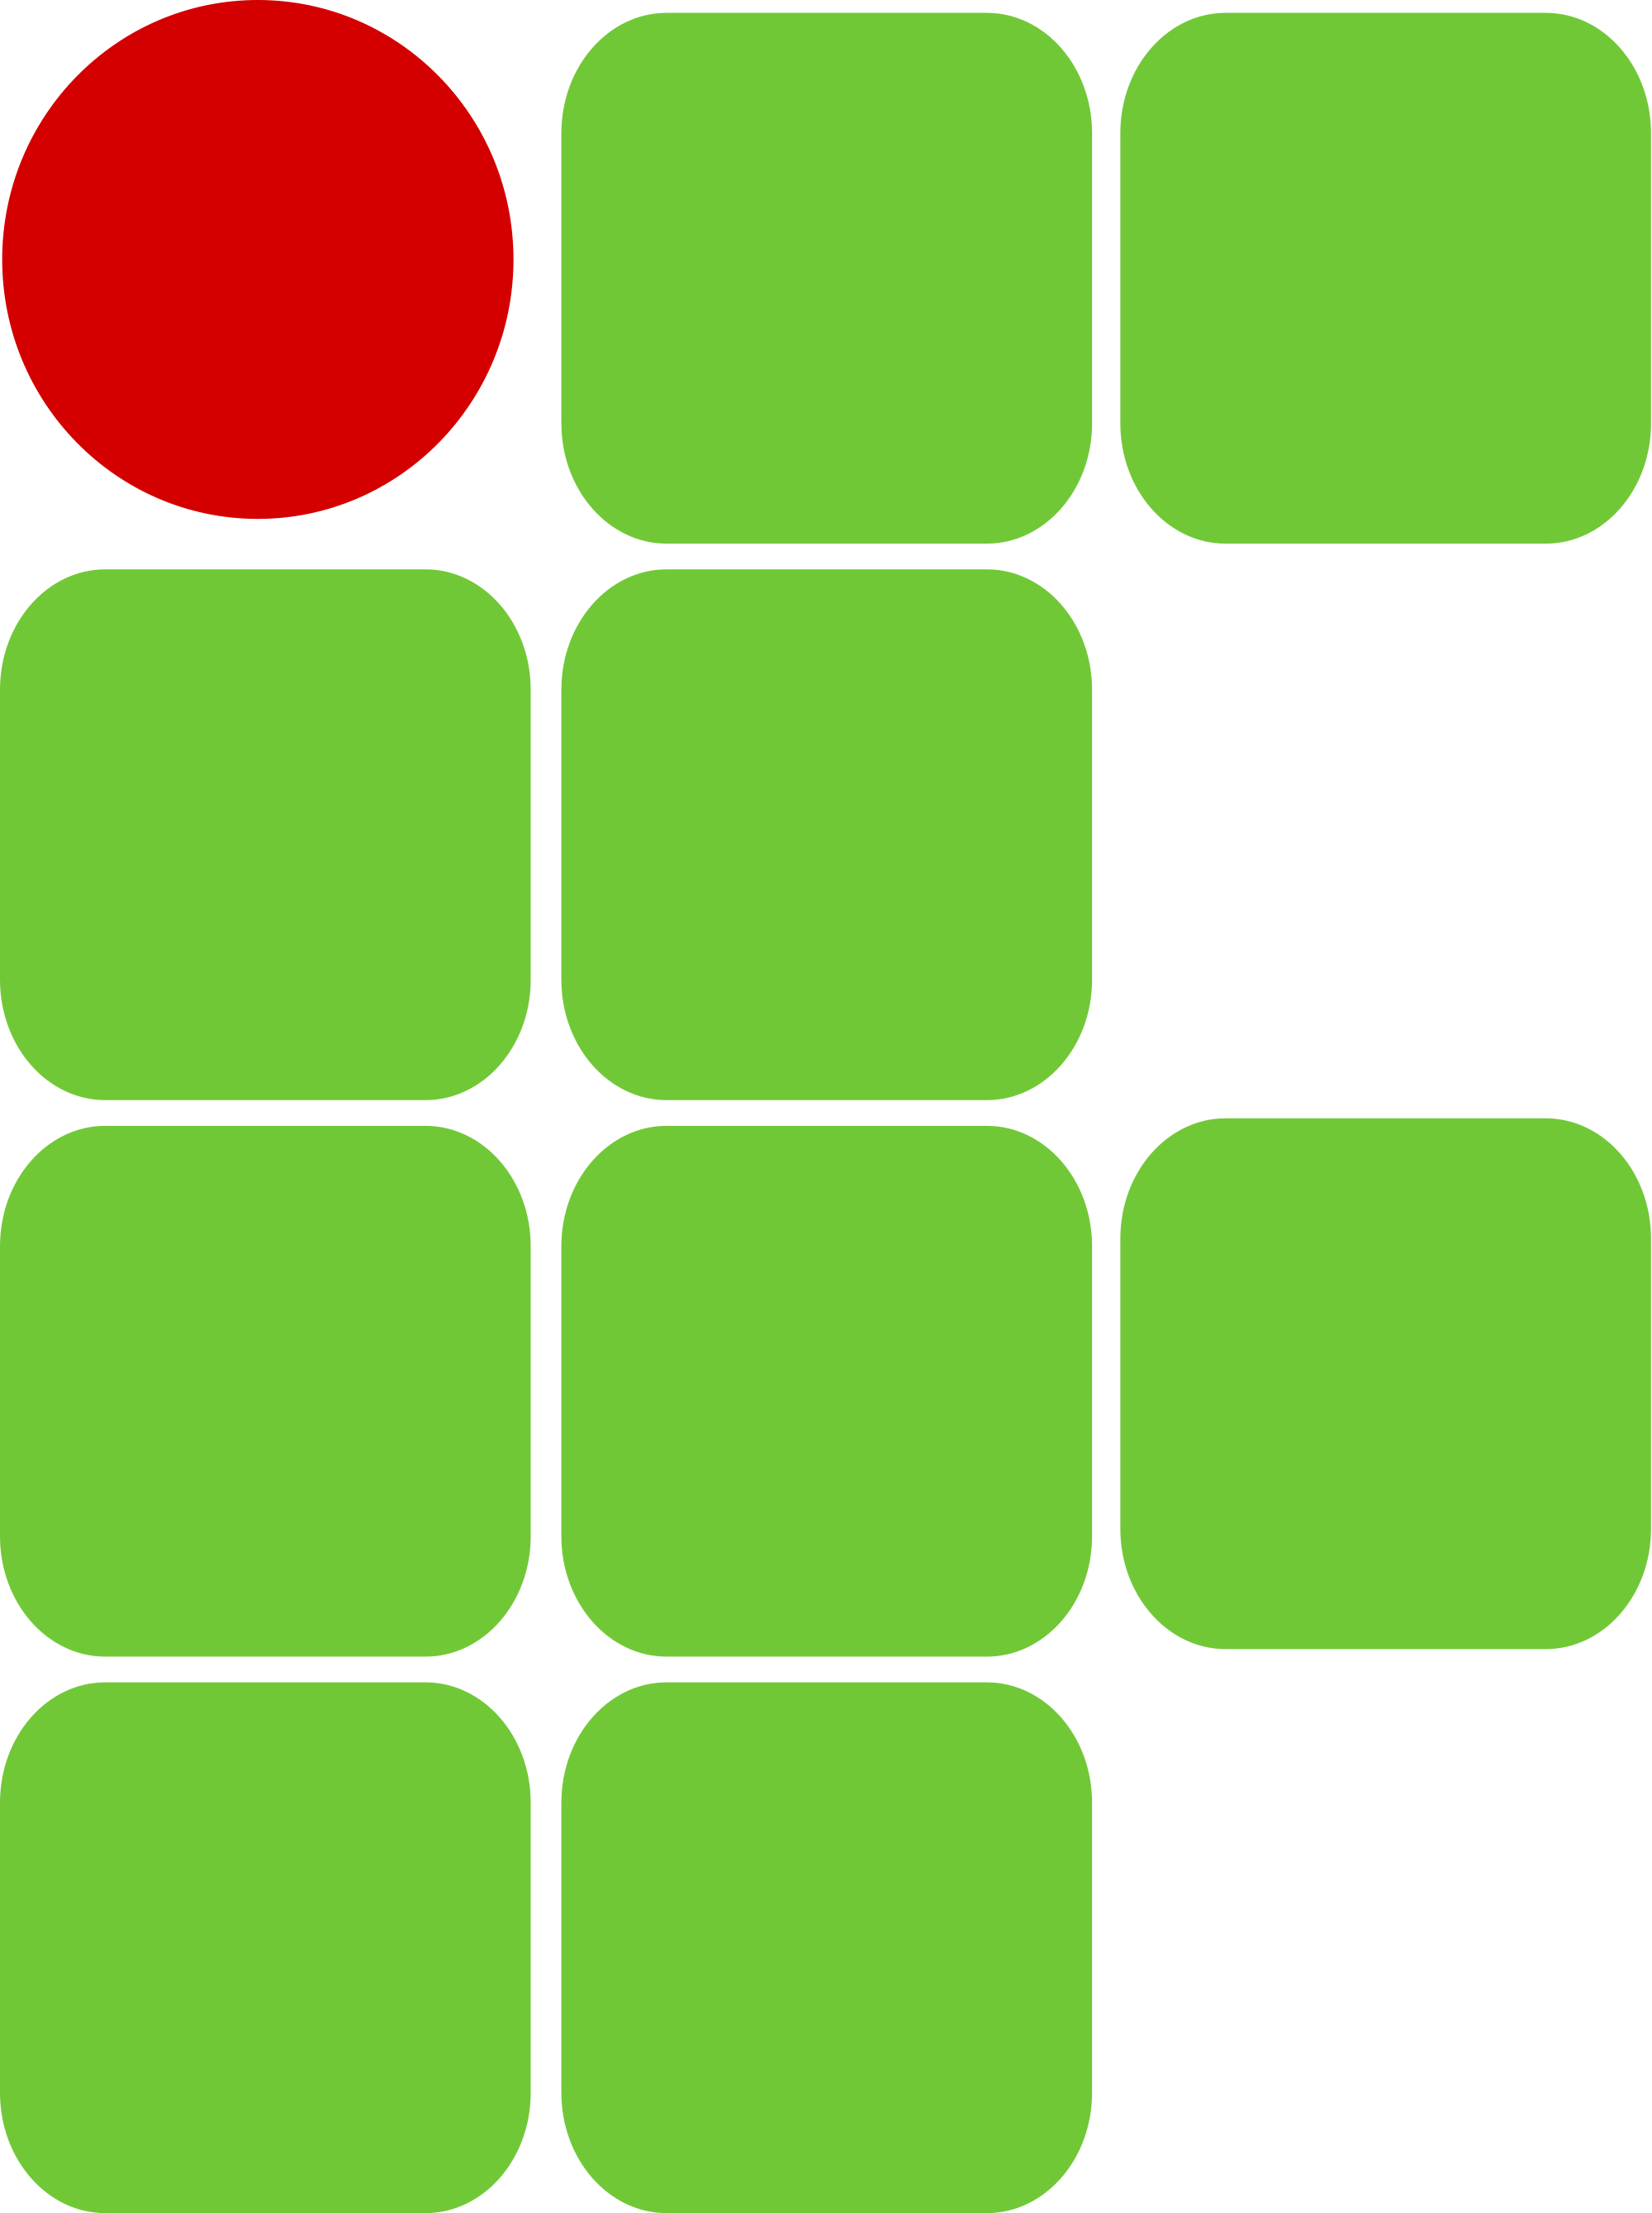
\includegraphics[height=0.7cm]{figs/logo.png}
\end{textblock*}
}

\setcounter{framenumber}{0}


% ----------------------------------------- %

\section*{Agenda}
%\frame{\tableofcontents}

 \begin{frame}{Agenda}
 
  \tableofcontents[pausesections, hideallsubsections]
   
\end{frame}

% --------------------------------------------------- %
%                      Slides                         %
% --------------------------------------------------- %
\section{Panorama}
\begin{frame}{Panorama geral}

Texto normal, \alert{Texto alerta},  \exemple{Texto exemplo}, \emph{Ênfase}
\begin{columns}

\begin{column}{0.5\textwidth}

\begin{block}{Padrão}
  \begin{itemize}
  	\item ...
  \end{itemize}
\end{block}

\pause

\begin{exampleblock}{Exemplo}
  \begin{itemize}
  	\item ...
  \end{itemize}
\end{exampleblock}

\pause

\begin{alertblock}{Alerta}
  \begin{itemize}
  	\item ...
  \end{itemize}
\end{alertblock}

\end{column}


\pause
\begin{column}{0.5\textwidth}

\boxpurple{
\centering
Roxo}

\boxorange{
\centering
Laranja}

\boxgrey{
\centering
Cinza}

% \begin{tcolorbox}[tablegreen,tabularx={X||Y|Y|Y|Y||Y}, boxrule=0.5pt, title=My price table]
% Color & Price 1  & Price 2  & Price 3 \\\hline\hline
% Red   & 10.00   & 20.00   &  30.00 \\\hline
% Green    & 20.00   & 30.00   &  40.00  \\\hline
% Blue    & 30.00   & 40.00   &  50.00 \\\hline\hline
% Orange  & 60.00   & 90.00   & 120.00 
% \end{tcolorbox}

\end{column}

\end{columns}
\end{frame}

\section{Blocos}
\begin{frame}{Tipo de blocos}

\begin{block}{Padrão}
\begin{itemize}
  \item Item 1
  \begin{itemize}
      \item Subitem 1
      \item Subitem 2
      \item Subitem 3
  \end{itemize}
  \item Item 2
  \item Item 3
\end{itemize}
\end{block}

\pause

\begin{exampleblock}{Exemplos}
    \begin{itemize}
      \item Item 1
      \item Item 2
      \item Item 3
    \end{itemize}
\end{exampleblock}

\pause

\begin{alertblock}{Alerta}
    \begin{itemize}
      \item Item 1
       \item Item 2
    \end{itemize}
\end{alertblock}
\end{frame}

\section{Boxes}

\begin{frame}{Boxes}

\boxyellow{
\centering
...}

\boxorange{
\centering
...}

\boxbrown{
\centering
...}

\boxpurple{
\centering
...}

\boxblue{
\centering
...}

\boxgrey{
\centering
...}

\boxgreen{
\centering
...}

\boxblack{
\centering
...}

\end{frame}



\section{Listas}

\subsection{Lista de items}

\begin{frame}{Items}

	\begin{itemize}[<+->]
		\item ...
    \item ...
    \item ...
  \end{itemize}
  
\end{frame} 

\subsection{Lista numerada}

\begin{frame}{Lista numerada}

	\begin{enumerate}[<+->]
		\item ...
    \item ...
    \item ...
  \end{enumerate}
  
\end{frame} 

\subsection{Lista descritiva} 

\begin{frame}{Lista descritiva} 

	\begin{description}
		\item [Opção 1:] ...
		\item [Opção 2:] ...
		\item [Opção 3:] ...
	\end{description}

\end{frame}


\section{Tabelas}

\begin{frame}{Tabelas 1}

\begin{columns}

  \begin{column}{0.5\textwidth}  

  \begin{tcolorbox}[tablered,tabularx={X||Y|Y}, boxrule=0.5pt, title=My price table]
  Couleur & Prix 1  & Prix 2 \\\hline\hline
  Rouge   & 10.00   & 20.00  \\\hline
  Vert    & 20.00   & 30.00  \\\hline
  Bleu    & 30.00   & 40.00  \\\hline\hline
  Orange  & 60.00   & 90.00 
  \end{tcolorbox}
  
  \begin{tcolorbox}[tableorange,tabularx={X||Y|Y}, boxrule=0.5pt, title=My price table]
  Couleur & Prix 1  & Prix 2 \\\hline\hline
  Rouge   & 10.00   & 20.00  \\\hline
  Vert    & 20.00   & 30.00  \\\hline
  Bleu    & 30.00   & 40.00  \\\hline\hline
  Orange  & 60.00   & 90.00 
  \end{tcolorbox}
  
  \end{column}

  \begin{column}{0.5\textwidth}
  
  \begin{tcolorbox}[tableblue,tabularx={X||Y|Y}, boxrule=0.5pt, title=My price table]
  Couleur & Prix 1  & Prix 2 \\\hline\hline
  Rouge   & 10.00   & 20.00  \\\hline
  Vert    & 20.00   & 30.00  \\\hline
  Bleu    & 30.00   & 40.00  \\\hline\hline
  Orange  & 60.00   & 90.00 
  \end{tcolorbox}
  
  \begin{tcolorbox}[tableyellow,tabularx={X||Y|Y}, boxrule=0.5pt, title=My price table]
  Couleur & Prix 1  & Prix 2 \\\hline\hline
  Rouge   & 10.00   & 20.00  \\\hline
  Vert    & 20.00   & 30.00  \\\hline
  Bleu    & 30.00   & 40.00  \\\hline\hline
  Orange  & 60.00   & 90.00 
  \end{tcolorbox}
  
  \end{column}

\end{columns}
\end{frame}
  
\begin{frame}{Tabelas 2}
\begin{columns}

  \begin{column}{0.5\textwidth} 
  
  
  \begin{tcolorbox}[tablegrey,tabularx={X||Y|Y}, boxrule=0.5pt, title=My price table]
  Couleur & Prix 1  & Prix 2 \\\hline\hline
  Rouge   & 10.00   & 20.00  \\\hline
  Vert    & 20.00   & 30.00  \\\hline
  Bleu    & 30.00   & 40.00  \\\hline\hline
  Orange  & 60.00   & 90.00 
  \end{tcolorbox}
  
  \begin{tcolorbox}[tablebrown,tabularx={X||Y|Y}, boxrule=0.5pt, title=My price table]
  Couleur & Prix 1  & Prix 2 \\\hline\hline
  Rouge   & 10.00   & 20.00  \\\hline
  Vert    & 20.00   & 30.00  \\\hline
  Bleu    & 30.00   & 40.00  \\\hline\hline
  Orange  & 60.00   & 90.00 
  \end{tcolorbox}

  \end{column}

  \begin{column}{0.5\textwidth}  

  \begin{tcolorbox}[tablepurple,tabularx={X||Y|Y}, boxrule=0.5pt, title=My price table]
  Couleur & Prix 1  & Prix 2 \\\hline\hline
  Rouge   & 10.00   & 20.00  \\\hline
  Vert    & 20.00   & 30.00  \\\hline
  Bleu    & 30.00   & 40.00  \\\hline\hline
  Orange  & 60.00   & 90.00 
  \end{tcolorbox}
  
  \begin{tcolorbox}[tableblack,tabularx={X||Y|Y}, boxrule=0.5pt, title=My price table]
  Couleur & Prix 1  & Prix 2 \\\hline\hline
  Rouge   & 10.00   & 20.00  \\\hline
  Vert    & 20.00   & 30.00  \\\hline
  Bleu    & 30.00   & 40.00  \\\hline\hline
  Orange  & 60.00   & 90.00 
  \end{tcolorbox}
  
  \end{column}

\end{columns}
\end{frame}
  

\section{Figuras}

\begin{frame}{Exemplo de figura} 

\begin{figure}
\centering
\caption{Reitoria IFMG.}
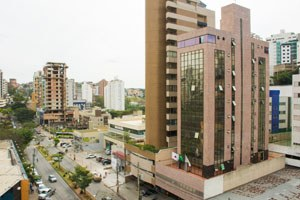
\includegraphics[width=0.8\linewidth]{figs/reitoria.jpeg}

\end{figure}

\end{frame}

\section{Equações e códigos}
\subsection{Equações}
\begin{frame}
\frametitle{Exemplos de equações}


\begin{block}{Exemplo de equação numerada}
\begin{align}
    \frac{\partial}{\partial \theta_k}J(\theta) 
        &= \frac{\partial}{\partial \theta_k}\Bigg[\frac{1}{m}\sum_{k=1}^m log(1+e^{-y^{(i)}\theta^Tx^{(i)}})\Bigg] \\
        &= \frac{1}{m}\sum_{k=1}^m \frac{1}{1+e^{-y^{(i)}\theta^Tx^{(i)}}}y^{(i)}x_k^{(i)} \\
        &= -\frac{1}{m}\sum_{k=1}^m h_\theta(-y^{(i)}x^{(i)})y^{(i)}x_k^{(i)}        
\end{align}
\end{block}
\begin{block}{Exemplo de equação não numerada}
    \begin{equation*}
        y(t) = Ax(t) + Bu(t)
    \end{equation*}
\end{block}

\end{frame}

\subsection{Programação}
\begin{frame}[fragile]

\frametitle{Código de exemplo}



\begin{block}{Código}
\begin{lstlisting}
def code():
  # test comments #1    
  if True:
    for _ in range(5):
      print("Hello World 5 times")
  return None     
\end{lstlisting}
\end{block}

\begin{lstlisting}[backgroundcolor = \color{lightgray}]
def code():
  # test comments #1    
  if True:
    for _ in range(5):
      print("Hello World 5 times")
  return None     
\end{lstlisting}

\end{frame}


\begin{frame}{Arquivo .py}
    \begin{block}{Código direto de um arquivo python}
        \inputminted{python}{codigos/codigo.py}
    \end{block}
    
    \boxorange{
        \centering
        Interessante
    }
\end{frame}

\end{document}
